\documentclass{ime-beamer}
\usepackage[portuges]{babel}
\usepackage[utf8]{inputenc}
\usepackage{graphicx}
\usepackage[portuguese]{algorithm2e}% Para escrever algorítimos
\usepackage{listings}			% Para usar \lstinputlisting e incluir código
\usepackage{subcaption}			% Para usar \begin{subfigure} e colocar figuras (a) e (b) lado a lado
\usepackage{multicol}

\title[Técnicas de IA aplicadas ao futebol de robôs]{%
  Técnicas de IA Aplicadas a Sistemas Multiagentes Cooperativos e Competitivos
}
\author[Jan Segre\and Victor Bramigk]{%
  Jan Segre\\
  Victor Bramigk\\
  Paulo F. F. Rosa (Orientador)\\
  Bruno Madeira (Co-orientador)
}

% as imagens ficam nesse diretório
\graphicspath{{img/}}

\begin{document}
\frame{\maketitle}

\frame{%
  \frametitle{Roteiro}
  \tableofcontents
}

\section{Introdução}
\frame{%
  \frametitle{Robocup}
  \begin{block}{}
    \begin{figure}
      \centering
      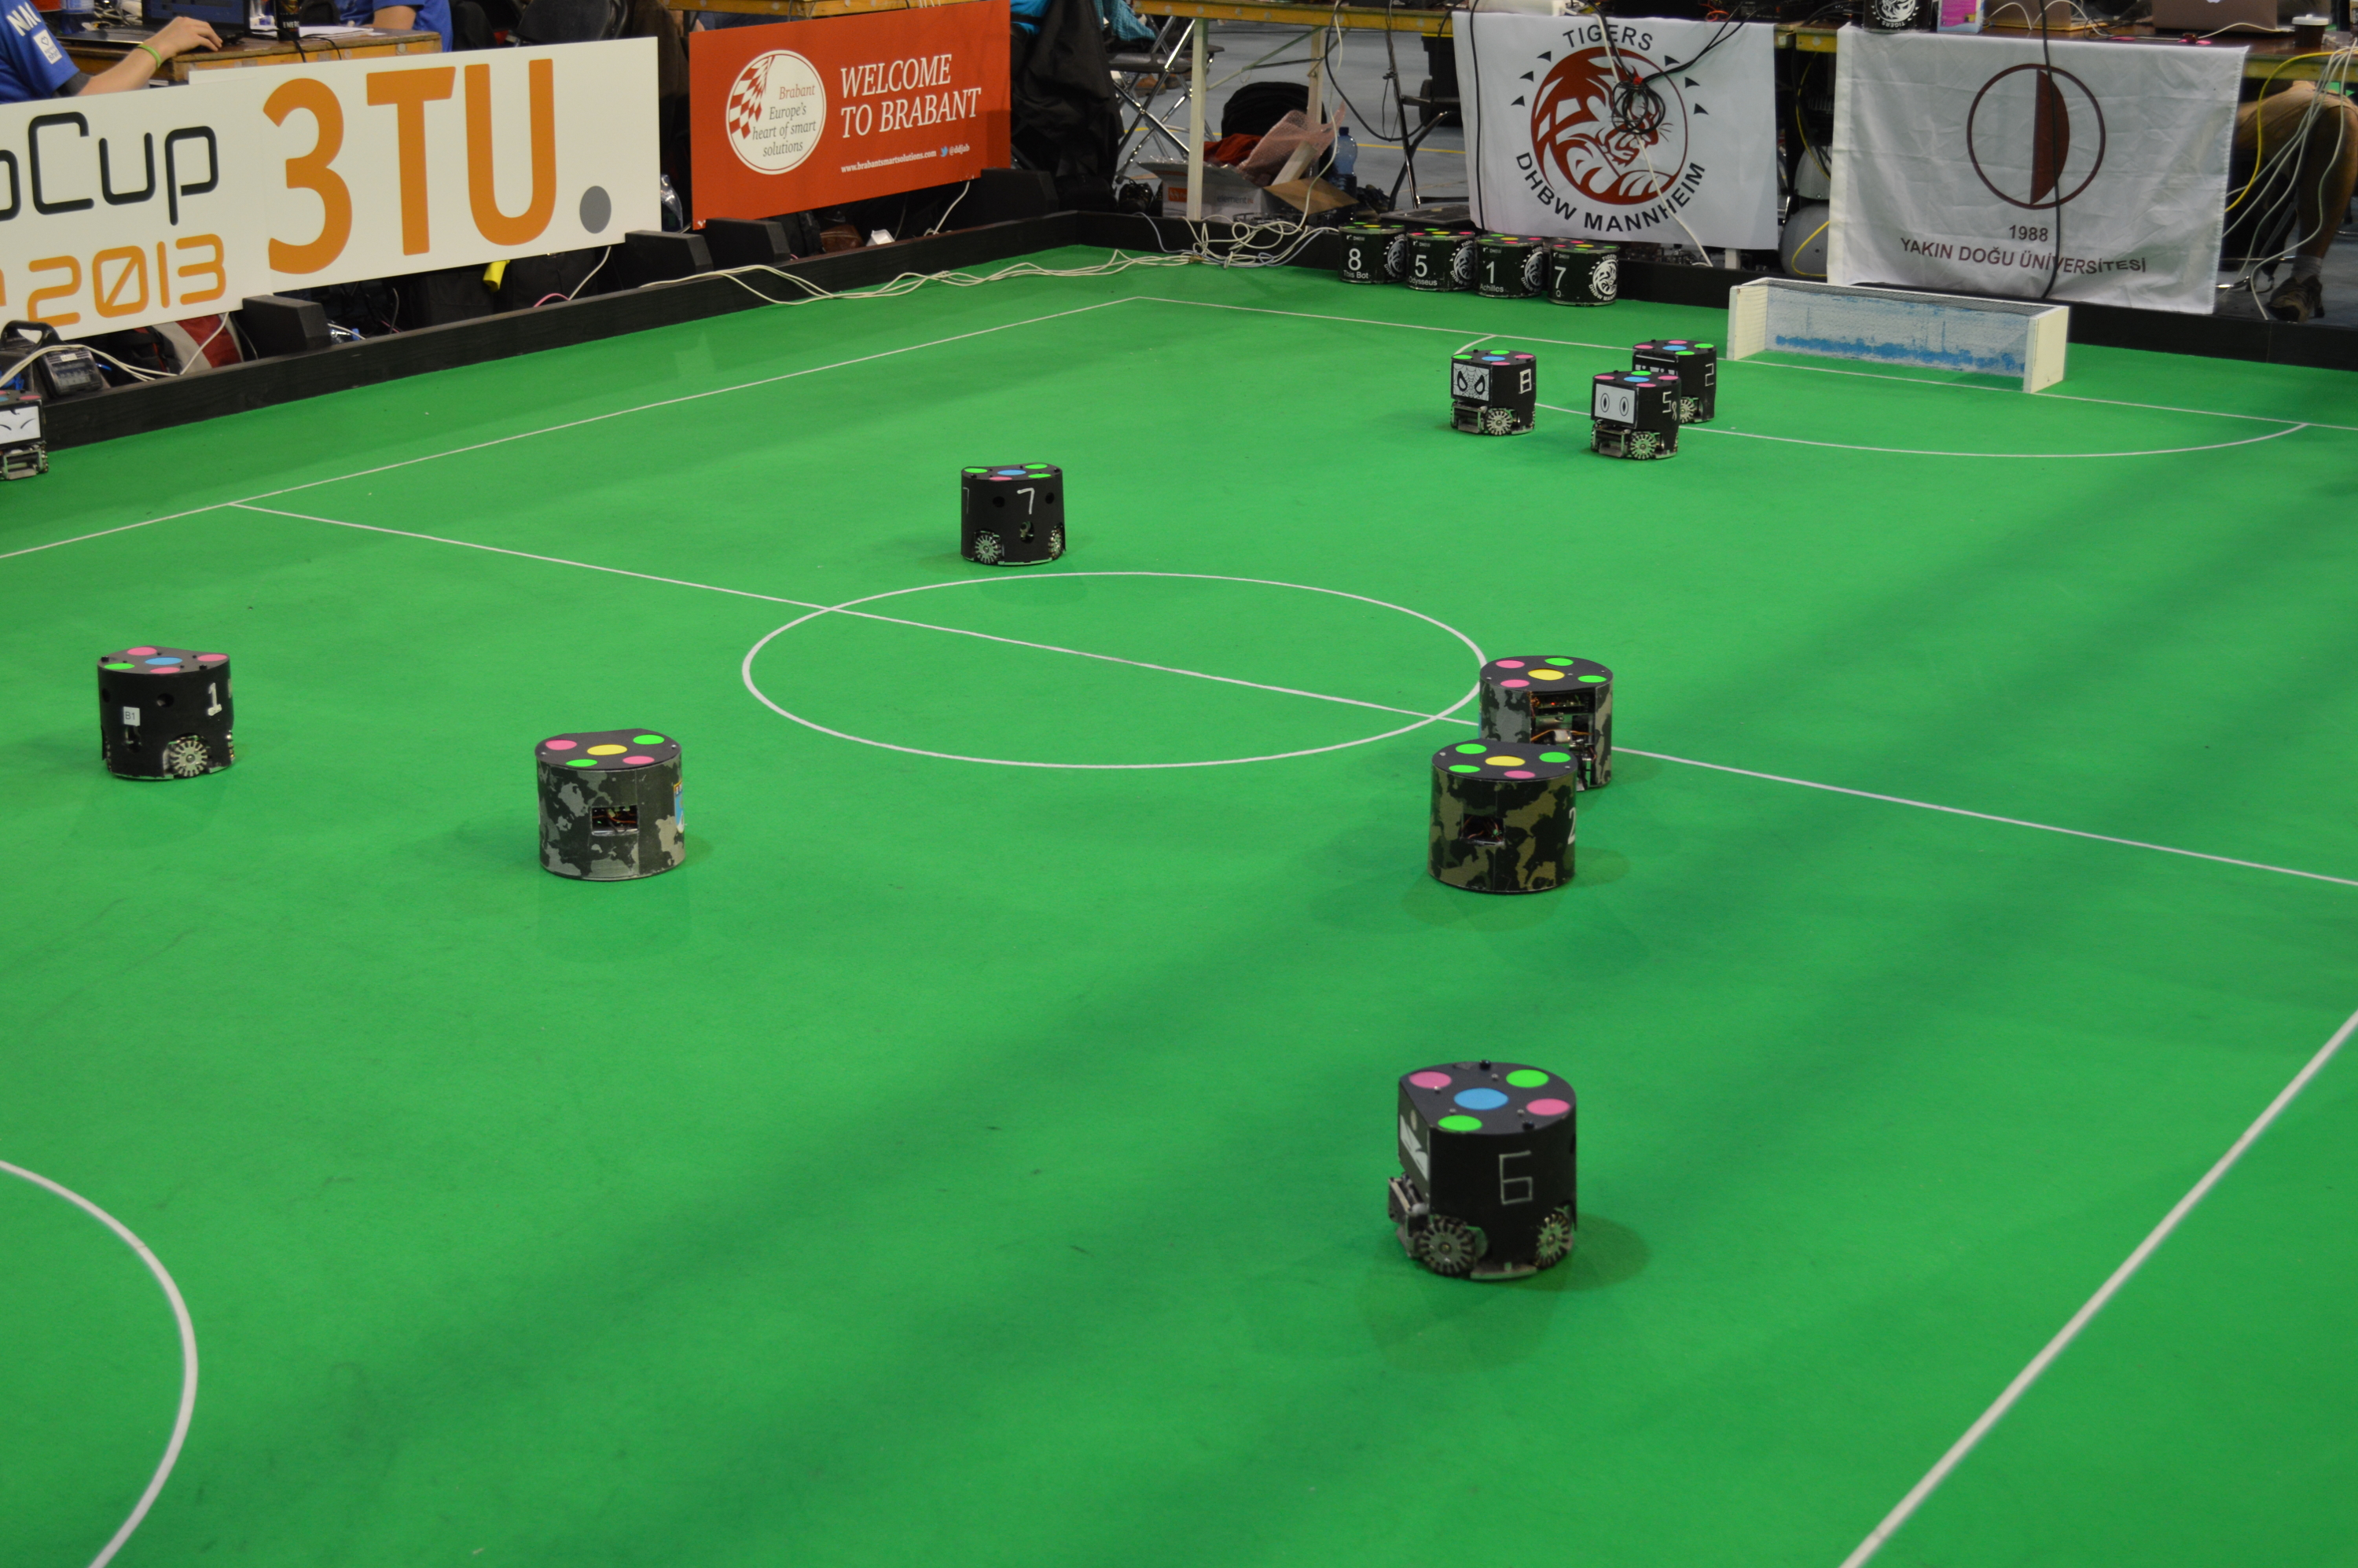
\includegraphics[width=0.7\linewidth]{robocup2013}
      \caption{Imagem da SSL \textit{RoboCup} 2013 em Eindhoven, na Holanda}\label{fig:robocup2013}
    \end{figure}
  \end{block}
}

\section{Minimax}
\frame{%
  \frametitle{Minimax}
  \begin{block}{}
    \centering
    Regra de decisão para minimizar a perda máxima.

    Se aplica a um jogo $\Gamma=\langle A,B,H\rangle$ quando:

    \begin{gather}
      v=\max_{a\in A}\min_{b\in B}H(a,b)=\min_{b\in B}\max_{a\in A}H(a,b)\label{eq:req}
    \end{gather}
  \end{block}
}
\frame{%
  \frametitle{Minimax}
  \begin{block}{}
    \begin{figure}[H]
      \centering
      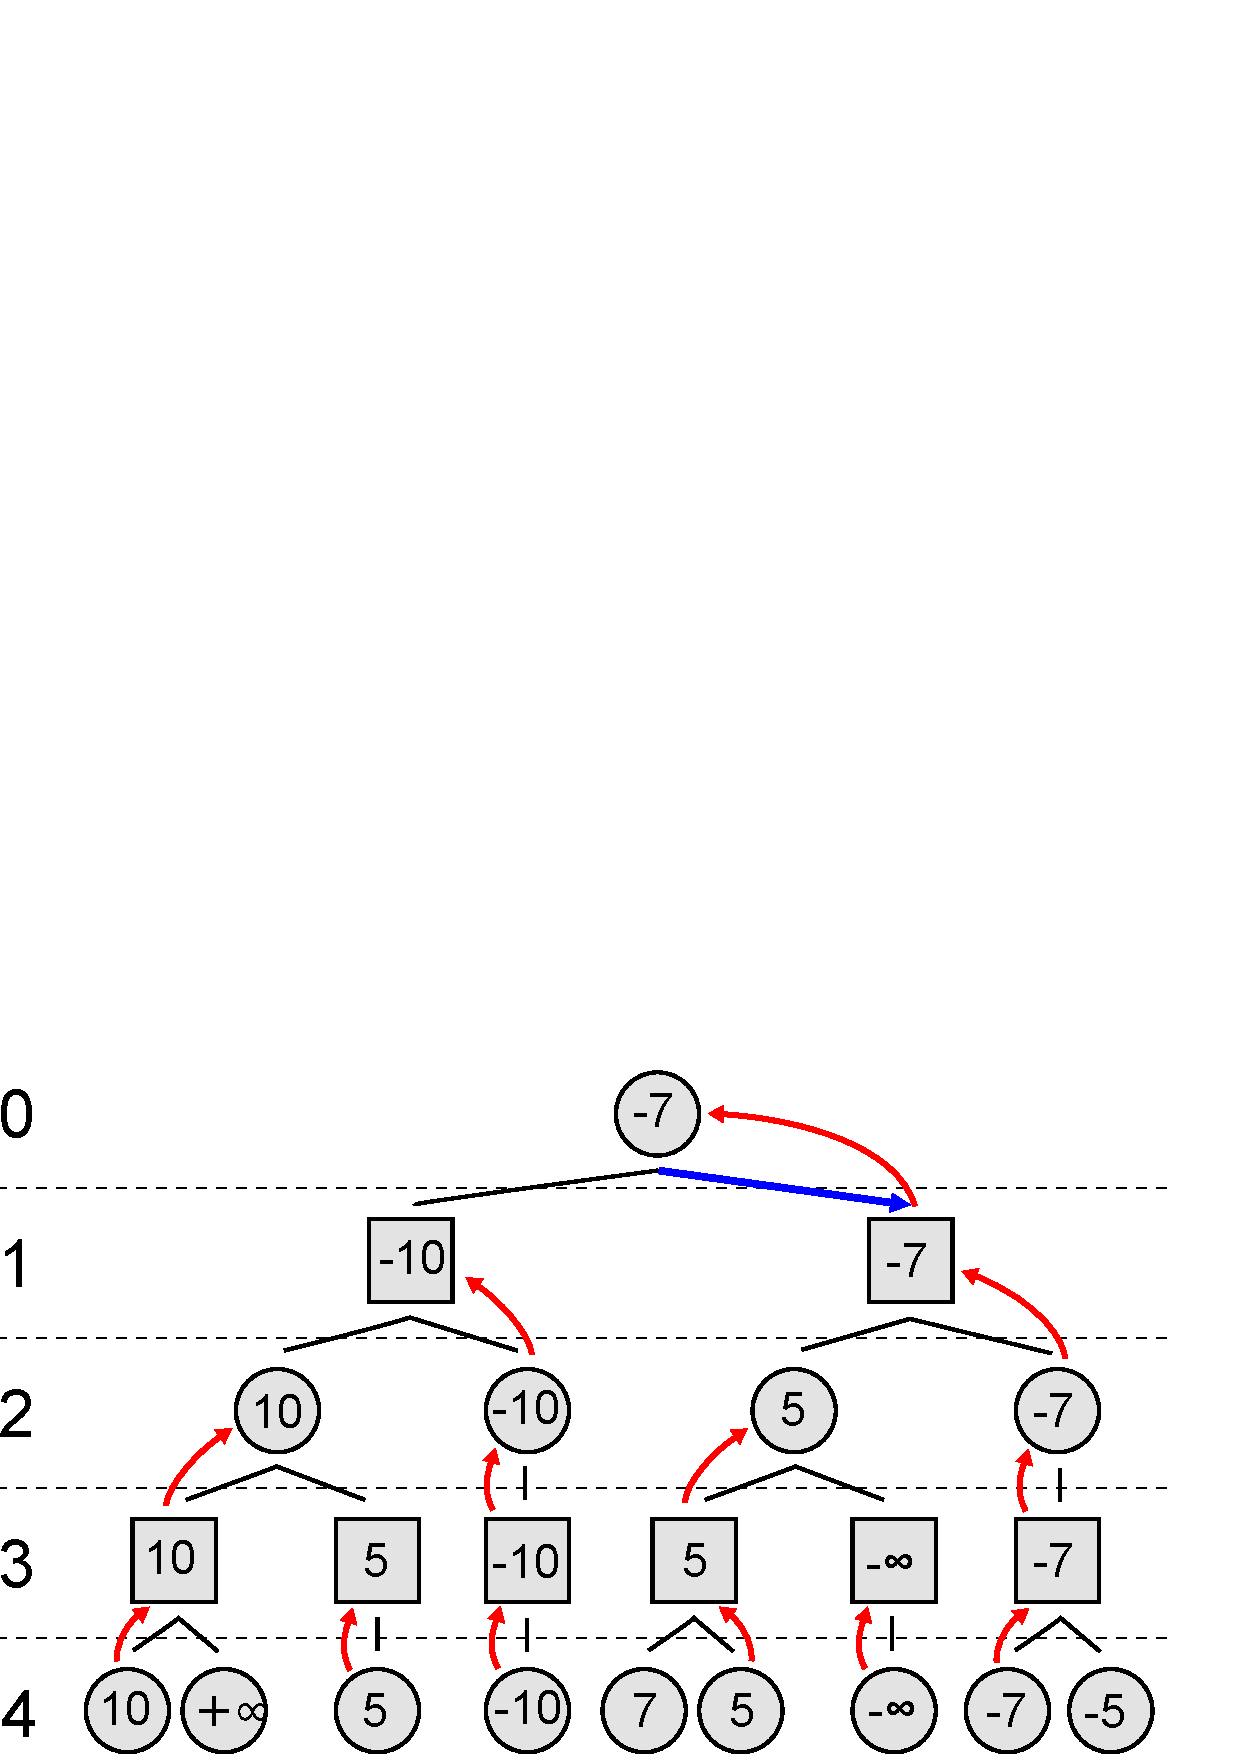
\includegraphics[width=0.7\linewidth]{minimax-tree}
      \caption{Exemplo de árvore de decisão com Minimax.}\label{fig:minimax-tree}
    \end{figure}
  \end{block}
}

\section{Mapeamento para um jogo discreto}
\frame{%
  \frametitle{Mapeamento para um jogo discreto}
  \begin{block}{}
    \centering
    Mapear um jogo contínuo em tempo e espaço para um jogo discreto em pelo
    menos no tempo, isto é, jogadas bem definidas.
  \end{block}
}
\frame{%
  \frametitle{Mapeamento para um jogo discreto}
  \begin{block}{}
    \centering
    Mapeamento proposto:

    \begin{itemize}
      \item Ação de um time com a bola é uma lista de:
        \begin{itemize}
          \item robô sem a bola:
            \begin{itemize}
              \item $Move(x, y)$
            \end{itemize}
          \item robô com a bola:
            \begin{itemize}
              \item $Kick(x, y)$
              \item $Pass(r)$
            \end{itemize}
        \end{itemize}
      \item Ação de um time sem a bola é uma lista de:
        \begin{itemize}
          \item $Move(x, y)$
        \end{itemize}
    \end{itemize}
  \end{block}
}

\section{Lições Aprendidas com implementações Anteriores}

\frame{%
  \frametitle{Lições Aprendidas com implementações Anteriores}
  \begin{block}{}
    \textbf{Abordagens}
    \begin{itemize}
      \item Heurística pura
      \item Otimização
      \item Baseado em jogos
      \item Otimização com modelagem do oponente
    \end{itemize}
  \end{block}
  \begin{block}{}
    \textbf{Longo prazo}
    Jogos + modelagem do oponente $\longrightarrow$ otimização
  \end{block}
}

\frame{%
  \frametitle{Lições Aprendidas com implementações Anteriores}
  \begin{block}{}
    \centering
    \textbf{Propostas de solução}
    \begin{itemize}
      \item No jogo com robôs omnidirecionais não são necessárias
        as trajetórias elaboradas
      \item Aproximar a simulação física por um jogo de tabuleiro.
    \end{itemize}
  \end{block}
  \begin{block}{}
    \begin{itemize}
      \item minimax com simulador físico: custo computacional das simulações
      \item minimax com chaveamento de heurística: custo computacional
      \item Resultado: heurísticas puras
    \end{itemize}
  \end{block}
}

\frame{%
  \frametitle{Lições Aprendidas com implementações Anteriores}
  \begin{block}{}
    \centering
    \textbf{Minimax para robôs omnidirecionais}
    \begin{itemize}
        \small
      \item Pegar a bola parada, se o oponente não estiver mais próximo da bola que o
        nosso robô.
      \item Pegar a bola em movimento, se for possível, escolhendo um ponto aleatório
        da trajetória da bola.
      \item Passar a bola, se não tiver ninguém que possa interceptar a bola.
      \item Chutar a gol, se não tiver ninguém no caminho da bola.
      \item Deslocar-se para outro ponto escolhido aleatoriamente, se não tiver ninguém
        em seu caminho, ou utilizar a célula de Voronoi.
      \item Deslocar-se para o ponto escolhido na última jogada. (aprendizagem local)
    \end{itemize}
  \end{block}
}

\frame{%
  \frametitle{Lições Aprendidas com implementações Anteriores}
  \begin{block}{}
    \textbf{Problemas}
    \begin{itemize}
      \item Mapeamento do modelo conceitual para o controle dos robôs
      \item Time defensor na árvore minimax tem vantagem
    \end{itemize}
  \end{block}
  \begin{block}{}
    \textbf{Ideias}
    \begin{itemize}
      \item Desacoplamento do comportamento dos jogadores para melhorar o
        aproveitamento da CPU\@.
      \item Definir algumas jogadas de movimento com finalidade especifica,
        (e.g., bloquear a bola defensivamente). Problema: tempo de processamento
    \end{itemize}
  \end{block}
}
\frame{%
  \frametitle{Lições Aprendidas com implementações Anteriores}
  \begin{block}{}
    \textbf{Considerações}
    \begin{itemize}
      \item Substituição das jogadas do oponente por jogadas aprendidas
        aumenta a efetividade das jogadas, e permite um maior tempo de
        planejamento
      \item Problema complexo
    \end{itemize}
  \end{block}
}

\section{Prova de Conceito}
\frame{%
  \frametitle{Prova de Conceito}
  \begin{block}{}
    \textbf{Frameworks}
    \begin{itemize}
      \item Protobuf (protocolo)
      \item Zmq (comunicação)
      \item pyroboime (máquinas de estados)
    \end{itemize}
  \end{block}
}
\frame{%
  \frametitle{Prova de Conceito}
  \begin{block}{}
    \textbf{Protocolo}
    \begin{itemize}
      \item int robot\_id
      \item enum Type type \{ MOVE, PASS, KICK\}
      \item Move move $\longrightarrow$ x, y
      \item Pass pass $\longrightarrow$ robot\_id
      \item Kick kick $\longrightarrow$ x, y
    \end{itemize}
  \end{block}
}
\frame{%
  \frametitle{Prova de Conceito}
  \begin{description}
    \begin{multicols}{2}
      \item command 3 move 0 0
      \item sleep 5
      \item command 2 move 1 1
      \item sleep 5
      \item command 3 pass 2
      \item sleep 4
      \item command 2 pass 3
      \item sleep 3
      \item command 4 move 1 0
      \item sleep 3
      \item command 3 pass 4
      \item sleep 3
      \item command 4 kick 3 0
      \item sleep 6
      \item command 4 move 1 -1
      \item sleep 300
    \end{multicols}
  \end{description}
}

\section{Cronograma}
\frame{%
  \frametitle{Cronograma}
  \begin{table}[Ht!]
    \begin{center}
      \begin{tabular}{|c|c|c|c|c|c|c|c|c|c|}
        \hline
        Data                   & Ago & Set & 0ut & Nov & Fev & Mar & Abr & Mai \\
        \hline
        \small{Modelagem do}   &  x  &  x  &     &     &     &     &     &     \\
        \small{mapeamento}     &     &     &     &     &     &     &     &     \\
        \hline
        \small{Prova de}       &     &     &  x  &  x  &     &     &     &     \\
        \small{conceito}       &     &     &     &     &     &     &     &     \\
        \hline
        \small{Implementação}  &     &     &  x  &  x  &     &     &     &     \\
        \small{da arquitetura} &     &     &     &     &     &     &     &     \\
        \hline
        \small{Implementação}  &     &     &     &     &  x  &  x  &  x  &     \\
        \small{do algoritmo}   &     &     &     &     &     &     &     &     \\
        \hline
        \small{Otimização}     &     &     &     &     &     &     &     &   x \\
        \small{do algoritmo}   &     &     &     &     &     &     &     &     \\
        \hline
      \end{tabular}
    \end{center}
  \end{table}
}

\end{document}
% vim: tw=80 et ts=2 sw=2 sts=2
